% The document class supplies options to control rendering of some standard
% features in the result.  The goal is for uniform style, so some attention 
% to detail is *vital* with all fields.  Each field (i.e., text inside the
% curly braces below, so the MEng text inside {MEng} for instance) should 
% take into account the following:
%
% - author name       should be formatted as "FirstName LastName"
%   (not "Initial LastName" for example),
% - supervisor name   should be formatted as "Title FirstName LastName"
%   (where Title is "Dr." or "Prof." for example),
% - degree programme  should be "BSc", "MEng", "MSci", "MSc" or "PhD",
% - dissertation title should be correctly capitalised (plus you can have
%   an optional sub-title if appropriate, or leave this field blank),
% - dissertation type should be formatted as one of the following:
%   * for the MEng degree programme either "enterprise" or "research" to
%     reflect the stream,
%   * for the MSc  degree programme "$X/Y/Z$" for a project deemed to be
%     X%, Y% and Z% of type I, II and III.
% - year              should be formatted as a 4-digit year of submission
%   (so 2014 rather than the academic year, say 2013/14 say).

\documentclass[ oneside,% the name of the author
                    author={George Herbert},
                % the degree programme: BSc, MEng, MSci or MSc.
                    degree={MSci},
                % the dissertation    title (which cannot be blank)
                     title={Video Diffusion Models for Climate Simulations},
                % the dissertation subtitle (which can    be blank)
                  subtitle={}]{dissertation}

\begin{document}

% =============================================================================

% This macro creates the standard UoB title page by using information drawn
% from the document class (meaning it is vital you select the correct degree 
% title and so on).

\maketitle

% After the title page (which is a special case in that it is not numbered)
% comes the front matter or preliminaries; this macro signals the start of
% such content, meaning the pages are numbered with Roman numerals.

\frontmatter


%\lstlistoflistings

% The following sections are part of the front matter, but are not generated
% automatically by LaTeX; the use of \chapter* means they are not numbered.

% -----------------------------------------------------------------------------

\chapter*{Abstract}

% {\bf A compulsory section, of at most 300 words} 
% \vspace{1cm} 

% \noindent
% This section should pr\'{e}cis the project context, aims and objectives,
% and main contributions (e.g., deliverables) and achievements; the same 
% section may be called an abstract elsewhere.  The goal is to ensure the 
% reader is clear about what the topic is, what you have done within this 
% topic, {\em and} what your view of the outcome is.

% The former aspects should be guided by your specification: essentially 
% this section is a (very) short version of what is typically the first 
% chapter. If your project is experimental in nature, this should include 
% a clear research hypothesis.  This will obviously differ significantly
% for each project, but an example might be as follows:

% \begin{quote}
% My research hypothesis is that a suitable genetic algorithm will yield
% more accurate results (when applied to the standard ACME data set) than 
% the algorithm proposed by Jones and Smith, while also executing in less
% time.
% \end{quote}

% \noindent
% The latter aspects should (ideally) be presented as a concise, factual 
% bullet point list.  Again the points will differ for each project, but 
% an might be as follows:

% \begin{quote}
% \noindent
% \begin{itemize}
% \item I spent $120$ hours collecting material on and learning about the 
%       Java garbage-collection sub-system. 
% \item I wrote a total of $5000$ lines of source code, comprising a Linux 
%       device driver for a robot (in C) and a GUI (in Java) that is 
%       used to control it.
% \item I designed a new algorithm for computing the non-linear mapping 
%       from A-space to B-space using a genetic algorithm, see page $17$.
% \item I implemented a version of the algorithm proposed by Jones and 
%       Smith in [6], see page $12$, corrected a mistake in it, and 
%       compared the results with several alternatives.
% \end{itemize}
% \end{quote}

% -----------------------------------------------------------------------------


\chapter*{Dedication and Acknowledgements}

% {\bf A compulsory section}
% \vspace{1cm} 

% \noindent
% It is common practice (although totally optional) to acknowledge any
% third-party advice, contribution or influence you have found useful
% during your work.  Examples include support from friends or family, 
% the input of your Supervisor and/or Advisor, external organisations 
% or persons who  have supplied resources of some kind (e.g., funding, 
% advice or time), and so on.


% -----------------------------------------------------------------------------

% This macro creates the standard UoB declaration; on the printed hard-copy,
% this must be physically signed by the author in the space indicated.

\makedecl



% -----------------------------------------------------------------------------

% LaTeX automatically generates a table of contents, plus associated lists 
% of figures and tables.  These are all compulsory parts of the dissertation.

\tableofcontents
\listoffigures
\listoftables

% -----------------------------------------------------------------------------



\chapter*{Ethics Statement}

% {\bf A compulsory section} 
% \vspace{1cm} 

% In almost every project, this will be one of the following statements:
%     \begin{itemize}
%         \item ``This project did not require ethical review, as determined by my supervisor, [fill in name]''; or
%         \item ``This project fits within the scope of ethics application 0026, as reviewed by my supervisor, [fill in name]''; or
%         \item ``An ethics application for this project was reviewed and approved by the faculty research ethics committee as application [fill in number]''.
%     \end{itemize}
    
% See Section 3.2 of the unit Handbook for more information. If something went wrong and none of those three statements apply, then you should instead explain what happened.


% -----------------------------------------------------------------------------

% \chapter*{Supporting Technologies}

% {\bf An optional section}
% \vspace{1cm} 

% \noindent
% This section should present a detailed summary, in bullet point form, 
% of any third-party resources (e.g., hardware and software components) 
% used during the project.  Use of such resources is always perfectly 
% acceptable: the goal of this section is simply to be clear about how
% and where they are used, so that a clear assessment of your work can
% result.  The content can focus on the project topic itself (rather,
% for example, than including ``I used \mbox{\LaTeX} to prepare my 
% dissertation''); an example is as follows:

% \begin{quote}
% \noindent
% \begin{itemize}
% \item I used the Java {\tt BigInteger} class to support my implementation 
%       of RSA.
% \item I used a parts of the OpenCV computer vision library to capture 
%       images from a camera, and for various standard operations (e.g., 
%       threshold, edge detection).
% \item I used an FPGA device supplied by the Department, and altered it 
%       to support an open-source UART core obtained from 
%       \url{http://opencores.org/}.
% \item The web-interface component of my system was implemented by 
%       extending the open-source WordPress software available from
%       \url{http://wordpress.org/}.
% \end{itemize}
% \end{quote}

% -----------------------------------------------------------------------------

\chapter*{Notation and Acronyms}

% {\bf An optional section}
% \vspace{1cm} 

% \noindent
% Any well written document will introduce notation and acronyms before
% their use, {\em even if} they are standard in some way: this ensures 
% any reader can understand the resulting self-contained content.  

% Said introduction can exist within the dissertation itself, wherever 
% that is appropriate.  For an acronym, this is typically achieved at 
% the first point of use via ``Advanced Encryption Standard (AES)'' or 
% similar, noting the capitalisation of relevant letters.  However, it 
% can be useful to include an additional, dedicated list at the start 
% of the dissertation; the advantage of doing so is that you cannot 
% mistakenly use an acronym before defining it.  A limited example is 
% as follows:

% \begin{quote}
% \noindent
% \begin{tabular}{lcl}
% AES                 &:     & Advanced Encryption Standard                                         \\
% DES                 &:     & Data Encryption Standard                                             \\
%                     &\vdots&                                                                      \\
% ${\mathcal H}( x )$ &:     & the Hamming weight of $x$                                            \\
% ${\mathbb  F}_q$    &:     & a finite field with $q$ elements                                     \\
% $x_i$               &:     & the $i$-th bit of some binary sequence $x$, st. $x_i \in \{ 0, 1 \}$ \\
% \end{tabular}
% \end{quote}


% =============================================================================

% After the front matter comes a number of chapters; under each chapter,
% sections, subsections and even subsubsections are permissible.  The
% pages in this part are numbered with Arabic numerals.  Note that:
%
% - A reference point can be marked using \label{XXX}, and then later
%   referred to via \ref{XXX}; for example Chapter\ref{chap:context}.
% - The chapters are presented here in one file; this can become hard
%   to manage.  An alternative is to save the content in seprate files
%   the use \input{XXX} to import it, which acts like the #include
%   directive in C.

\mainmatter


\chapter{Introduction}
\label{chap:introduction}

\chapter{Background}
\label{chap:background}

\section{Diffusion Models}
\label{sec:background_diffusion}

Diffusion models are 

Given observed datapoints $\mathbf{x}$, the goal of a generative model is to learn to model its true data distribution $q(\mathbf{x})$.

\subsection{Forward Diffusion Process}
\label{sec:background_diffusion_forward}

The \textit{forward diffusion process} is a Gaussian diffusion process that defines a sequence of increasingly noisy versions of $\mathbf{x}$, which we call the \textit{latent variables}:
\begin{align}
      \mathbf{z}=\{\mathbf{z}_t\mid t\in[0,1]\}
\end{align}
The forward process forms a conditional joint distribution $q(\mathbf{z}|\mathbf{x})$, whose marginal distributions of latent variables $\mathbf{z}_t$ given $\mathbf{x}\sim q(\mathbf{x})$ are given by:
\begin{align}
      q(\mathbf{z}_t|\mathbf{x})=\mathcal{N}\left(\mathbf{z}_t;\alpha_t\mathbf{x},\sigma_t^2\mathbf{I}\right)
      \label{eq:q_z_t_given_x}
\end{align}
where $\alpha_t$ and $\sigma_t$ are strictly positive scalar-valued functions of $t$. The joint distribution of latent variables $\mathbf{z}_r,\mathbf{z}_s,\mathbf{z}_t$ at subsequent timesteps $0\le r < s < t \le 1$ is Markovian:
\begin{align}
      q(\mathbf{z}_t|\mathbf{z}_s,\mathbf{z}_r)&=q(\mathbf{z}_t|\mathbf{z}_s)=\mathcal{N}\left(\mathbf{z}_t; \alpha_{t|s}\mathbf{z}_s, \sigma_{t|s}^2\mathbf{I}\right)
\end{align}
where $\alpha_{t|s}=\alpha_t\alpha_s^{-1}$ and $\sigma_{t|s}^2=\sigma_t^2-\alpha_{t|s}^2\sigma_s^2$. A full derivation of $q(\mathbf{z}_t|\mathbf{z}_s)$ is given in Appendix \ref{appx:diffusion_q_z_t_given_z_s}.

\subsection{Noise Schedule}
\label{sec:background_diffusion_noise_schedule}

We formalise the notion that $\mathbf{z}_t$ is increasingly noisy by defining the log signal-to-noise ratio
\begin{align}
      \lambda_t = \log\left( \frac{\alpha_t^2}{\sigma_t^2}\right)\in[\lambda_{\min}, \lambda_{\max}]
\end{align}
as a strictly monotonically decreasing function $f_{\lambda}$ of time $t\in[0, 1]$, known as the \textit{noise schedule}.

In this work, we use a truncated continuous-time version of the $\alpha$-cosine schedule \cite{IDDPM_Nichol}, introduced in its original discrete-time form by Nichol and Dhariwal \cite{IDDPM_Nichol}. The $\alpha$-cosine schedule was motivated by the fact that the `linear' schedule introduced in prior work by Ho et al. \cite{DDPM_Ho} causes $\alpha_t$ to fall to zero more quickly than is optimal. Nichol and Dhariwal empirically found that this induces too much noise in the latter stages of the forward diffusion process; as such, the latent variables $\mathbf{z}_t$ in these stages contribute little to sample quality. In response, they proposed the original discrete-time $\alpha$-cosine schedule. In this work, we use a continuous-time diffusion model and therefore use an adapted model described in \cite{Simple_Diffusion_Hoogeboom}. More formally, we define:
\begin{align}
      f_{\lambda}(t)=-2\log\left(\tan\left(\frac{\pi}{2}(t_0+t(t_1-t_0))\right)\right)
      \label{eq:f_lambda_alpha_cosine}
\end{align} 
where $t_0$ and $t_1$ truncate $f_{\lambda}(t)$ to the desired range $[\lambda_{\min}, \lambda_{\max}]$ for $t\in[0,1]$, and are themselves defined as:
\begin{align}
      t_0&=\frac{2}{\pi}\arctan\left(\exp\left(-\frac{1}{2}\lambda_{\max}\right)\right)\\
      t_1&=\frac{2}{\pi}\arctan\left(\exp\left(-\frac{1}{2}\lambda_{\min}\right)\right)
\end{align}
Figure \ref{fig:cosine_lambda_t} visualises how the log signal-to-noise ratio $\lambda_t\in[\lambda_{\min},\lambda_{\max}]$ varies with time $t\in[0,1]$ using the $\alpha$-cosine schedule detailed above.

\begin{figure}[htbp]
      \centering
      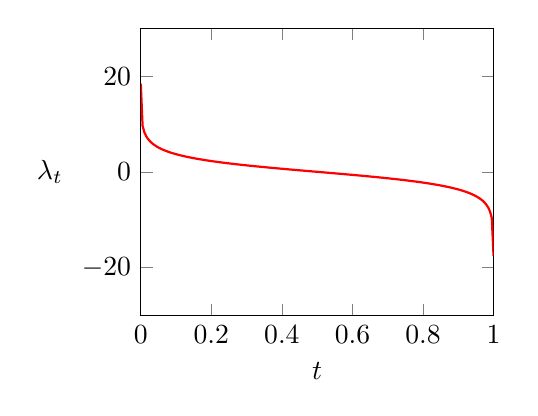
\begin{tikzpicture}
      \begin{axis}[
            xlabel=$t$,
            ylabel=$\lambda_t$,
            ylabel near ticks,
            xlabel near ticks,
            ylabel style={rotate=-90},
            xmin=0,
            xmax=1,
            ymin=-30,
            ymax=30,
            width=.5\linewidth]
      \addplot[color=red,thick,domain=-0.005:1.005,samples=200]{-2 * ln(tan(deg(pi / 2 * ((2 / pi * rad(atan(exp(-0.5 * 30)))) + x * ((2 / pi * rad(atan(exp(-0.5 * -30)))) - (2 / pi * rad(atan(exp(-0.5 * 30)))))))))};
      \end{axis}
      \end{tikzpicture}
      \caption{Relationship between time $t$ and the log signal-to-noise ratio $\lambda_t$ for the truncated continuous-time $\alpha$-cosine noise schedule $f_\lambda(t)$ as defined in Equation \ref{eq:f_lambda_alpha_cosine} with $\lambda_{\min}=-30$ and $\lambda_{\max}=30$. The horizontal axis is time $t\in[0,1]$; the vertical axis is $\lambda_t=f_\lambda(t)\in[\lambda_{\min},\lambda_{\max}]=[-30, 30]$.}
      \label{fig:cosine_lambda_t}
\end{figure}

We can compute $\alpha_t$ and $\sigma_t$ from either $\lambda_t$ or $t$ via the following equations:
\begin{alignat}{2}
      \alpha_t&=\sqrt{S(\lambda_t)}&&=\cos\left(\frac{\pi}{2}(t_0+t(t_1-t_0)\right)\label{eq:alpha_t_alpha_cosine}\\
      \sigma_t&=\sqrt{S(-\lambda_t)}&&=\sin\left(\frac{\pi}{2}(t_0+t(t_1-t_0)\right)\label{eq:sigma_t_alpha_cosine}
\end{alignat}
where $S$ is the sigmoid function. Figure \ref{fig:cosine_alpha_sigma} visualises how the values of $\alpha_t$ and $\sigma_t$ vary with time $t\in[0,1]$ using the $\alpha$-cosine schedule detailed above. Appendix \ref{appx:diffusion_cosine_noise_schedule} provides further details on the form of $f_\lambda$ and how we can derive the forms for $\alpha_t$ and $\sigma_t$.

\begin{figure}[htbp]
      \begin{subfigure}{0.5\textwidth}
            \begin{tikzpicture}
            \begin{axis}[
                  xlabel=$t$,
                  ylabel=$\alpha_t$,
                  ylabel near ticks,
                  xlabel near ticks,
                  ylabel style={rotate=-90},
                  xmin=0,
                  xmax=1,
                  ymin=0,
                  ymax=1,
                  width=\linewidth]
            \addplot[color=red,thick,domain=0:1,samples=100]{cos(deg(pi / 2 * ((2 / pi * rad(atan(exp(-0.5 * 30)))) + x * ((2 / pi * rad(atan(exp(-0.5 * -30)))) - (2 / pi * rad(atan(exp(-0.5 * 30))))))))};
            \end{axis}
            \end{tikzpicture}
      \end{subfigure}
      \begin{subfigure}{0.5\textwidth}
            \begin{tikzpicture}
            \begin{axis}[
                  xlabel=$t$,
                  ylabel=$\sigma_t$,
                  ylabel near ticks,
                  xlabel near ticks,
                  ylabel style={rotate=-90},
                  xmin=0,
                  xmax=1,
                  ymin=0,
                  ymax=1,
                  width=\linewidth]
            \addplot[color=red,thick,domain=0:1,samples=100]{sin(deg(pi / 2 * ((2 / pi * rad(atan(exp(-0.5 * 30)))) + x * ((2 / pi * rad(atan(exp(-0.5 * -30)))) - (2 / pi * rad(atan(exp(-0.5 * 30))))))))};
            \end{axis}
            \end{tikzpicture}
      \end{subfigure}
      \caption{Relationship between time $t$ and $\alpha_t$ (left) and $\sigma_t$ (right) for the same truncated continuous-time $\alpha$-cosine noise schedule as that in Figure \ref{fig:cosine_lambda_t}. The horizontal axis is time $t\in[0,1]$; the vertical axis is the value of $\alpha_t$ (left) and $\sigma_t$ (right).}
      \label{fig:cosine_alpha_sigma}
\end{figure}

\subsection{Generative Model}
\label{sec:background_diffusion_reverse}

The \textit{generative model} is a learned hierarchical model that matches the forward process running in reverse-time: in $T$ uniformly-spaced discrete timesteps, we sequentially generate latent variables, starting from $t=1$ and working backwards to $t=0$. More formally, our hierarchical generative model defines a joint distribution over latent variables:
\begin{align}
      p_\theta(\mathbf{z})=p(\mathbf{z}_1)\prod_{i=1}^T p_\theta(\mathbf{z}_{s(i)}|\mathbf{z}_{t(i)})
\end{align}
where $s(i)=(i - 1)\cdot T^{-1}$ and $t(i)=i\cdot T^{-1}$. For large enough $\lambda_{\max}$, $\mathbf{z}_0$ is almost noiseless, so learning a model $p_\theta(\mathbf{z}_0)$ is practically equivalent to learning a model $p_\theta(\mathbf{x})$. 

For sufficiently small $\lambda_{\min}$, $\mathbf{z}_1$ contains almost no information about $\mathbf{x}$. As such, there exists a distribution $p(\mathbf{z}_1)$ such that:
\begin{align}
      D_{KL}(q(\mathbf{z}_1|\mathbf{x})\Vert p(\mathbf{z_1}))\approx 0
\end{align}
where $D_{KL}$ is the Kullback--Leibler divergence. In this work, we use a variance-preserving diffusion model (i.e. $\alpha_t^2=1-\sigma_t^2$), and as such, we model $p(\mathbf{z}_1)$ as the multivariate standard Gaussian:
\begin{align}
      p(\mathbf{z}_1)=\mathcal{N}(\mathbf{z}_1;\mathbf{0}, \mathbf{I})
\end{align}

Once we have sampled $\mathbf{z}_1\sim p(\mathbf{z}_1)$, we use the discrete-time ancestral sampler \cite{DDPM_Ho} to sequentially generate each latent variable $\mathbf{z}_s$ from $\mathbf{z}_t$ where $0\le s < t \le 1$. The discrete-time ancestral sampler samples $\mathbf{z}_s\sim p_\theta(\mathbf{z}_s|\mathbf{z}_t)$ via:
\begin{align}
      p_\theta(\mathbf{z}_s|\mathbf{z}_t)&=q(\mathbf{z}_s|\mathbf{z}_t,\mathbf{x}=\hat{\mathbf{x}}_\theta(\mathbf{z}_t,\lambda_t))\\
      &=\mathcal{N}\left(\tilde{\boldsymbol\mu}_{s|t}(\mathbf{z}_t,\mathbf{x}=\hat{\mathbf{x}}_\theta(\mathbf{z}_t,\lambda_t)), \tilde{\sigma}_{s|t}\mathbf{I}\right)
\end{align}
where $\hat{\mathbf{x}}_\theta(\mathbf{z}_t,\lambda_t)$ is our denoised estimate of the original data $\mathbf{x}$ given latent $\mathbf{z}_t$ and log signal-to-noise ratio $\lambda_t$, and
\begin{align}
      \tilde{\boldsymbol\mu}_{s|t}(\mathbf{z}_t,\mathbf{x})&=\frac{\alpha_{t|s}\sigma_s^2}{\sigma_t^2}\mathbf{z}_t+\frac{\alpha_s\sigma_{t|s}^2}{\sigma_t^2}\mathbf{x}\\
      \tilde{\sigma}_{s|t}^2&=\frac{\sigma_{t|s}\sigma_s}{\sigma_t}
\end{align}

\subsection{Parameterisations}
\label{sec:background_diffusion_parameterisations}

In Section \ref{sec:background_diffusion_reverse}, we defined our generative model $p_\theta(\mathbf{x})$ using $\hat{\mathbf{x}}_\theta(\mathbf{z}_t,\lambda_t)$, which takes as input some noisy latent variable $\mathbf{z}_t$ and a log signal-to-noise ratio $\lambda_t$ and outputs a denoised estimate of the latent. Training a neural network to predict $\mathbf{x}\approx\hat{\mathbf{x}}_\theta(\mathbf{z}_t, \lambda_t)$ directly is referred to as the $\mathbf{x}$-prediction parameterisation, but is seldom adopted in the broader literature due to sub-optimal results \cite{DDPM_Ho}.Recent diffusion models have instead adopted different parameterisations, most commonly the $\boldsymbol\epsilon$-prediction parameterisation (e.g. \cite{DDPM_Ho,Cascaded_Ho,Imagen_Saharia}), wherein a neural network is instead trained to predict the noise $\boldsymbol\epsilon\approx\hat{\boldsymbol\epsilon}_\theta(\mathbf{z}_t,\lambda_t)$, from which we can compute a denoised estimate of noisy latent $\mathbf{z}_t$ via:
\begin{align}
      \hat{\mathbf{x}}_\theta(\mathbf{z}_t,\lambda_t)=\frac{1}{\alpha_t}\left(\mathbf{z}_t-\sigma_t\hat{\boldsymbol\epsilon}_\theta(\mathbf{z}_t, \lambda_t)\right)
\end{align}
In this work, we employ the $\mathbf{v}$-prediction parameterisation, introduced originally by Salimans and Ho \cite{Progressive_Distillation_Salimans}, and commonly employed in video diffusion models (e.g. \cite{VDM_Ho,Imagen_Video_Ho}). The $\mathbf{v}$-prediction parameterisation was originally introduced facilitate progressive distillation for faster sampling, though we utilise it here for its additional benefits highlighted by Ho et al. \cite{Imagen_Video_Ho}, namely faster convergence of sample quality and prevention of temporal colour shifting sometimes observed with $\boldsymbol\epsilon$-prediction video diffusion models. 

Formally, for a given datapoint $\mathbf{x}\sim q(\mathbf{x})$  we define the velocity of $\mathbf{z}_t\sim q(\mathbf{z}_t|\mathbf{x})$ as:
\begin{align}
      \mathbf{v}_t=\alpha_t\boldsymbol\epsilon - \sigma_t\mathbf{x}
\end{align}
where $\boldsymbol\epsilon\sim\mathcal{N}(\mathbf{0}, \mathbf{I})$ is multivariate standard Gaussian noise. We train our neural network $\hat{\mathbf{v}}_\theta(\mathbf{z}_t,\lambda_t)$ to minimise the following loss function, defined per datapoint $\mathbf{x}$ as:
\begin{align}
      \mathbb{E}_{\lambda\sim p_\Lambda(\lambda),\boldsymbol\epsilon\sim\mathcal{N}(\mathbf{0},\mathbf{I})}\left[\Vert\mathbf{v}_t-\hat{\mathbf{v}}_\theta(\mathbf{z}_t, \lambda_t)\Vert_2^2\right]
\end{align}
During discrete-time ancestral sampling, we convert our estimate $\mathbf{v}_t\approx\hat{\mathbf{v}}_\theta(\mathbf{z}_t,\lambda_t)$ into an estimate of the denoised latent $\mathbf{x}\approx\hat{\mathbf{x}}_\theta(\mathbf{z}_t,\lambda_t)$ via:
\begin{align}
      \hat{\mathbf{x}}(\mathbf{z}_t,\lambda_t)=\alpha_t\mathbf{z}_t-\sigma_t\hat{\mathbf{v}}_\theta(\mathbf{z}_t,\lambda_t)
\end{align}
Appendix \ref{appx:diffusion_v_prediction_parameterisation} provides further details on the $\mathbf{v}$-prediction parameterisation, including derivations of the velocity and denoised latent.

\subsection{Objective Function}
\label{sec:background_diffusion_objective}

Kingma and Gao \cite{Understanding_Diffusion_Objective_Kingma} discovered that diffusion models in the broader literature are optimised with various objectives that are almost all special cases of a weighted loss, which is defined per datapoint $\mathbf{x}$ as:
\begin{align}
      \mathcal{L}_w&=w(\lambda_{\min})\mathcal{L}(\lambda_{\min})+\frac{1}{2}\int_{\lambda_{\min}}^{\lambda_{\max}}w(\lambda)\mathbb{E}_{\boldsymbol\epsilon\sim\mathcal{N}(\mathbf{0},\mathbf{I})}\left[\Vert\boldsymbol\epsilon-\hat{\boldsymbol\epsilon}_\theta(\mathbf{z}_t,\lambda_t)\Vert_2^2\right]d\lambda\\
      &=w(\lambda_{\min})\mathcal{L}(\lambda_{\min})+\frac{1}{2}\mathbb{E}_{\lambda\sim p(\lambda),\boldsymbol\epsilon\sim\mathcal{N}(\mathbf{0},\mathbf{I})}\left[\frac{w(\lambda)}{p(\lambda)}\Vert\boldsymbol\epsilon-\hat{\boldsymbol\epsilon}(\mathbf{z}_t,\lambda_t)\Vert_2^2\right]
\end{align}
where $\mathcal{L}(\lambda)$ is the Kullback--Leibler divergence from the joint distributions $q$ to $p$ for a subset of timesteps from $t=f_\lambda^{-1}(\lambda)$ to $1$ for datapoint $\mathbf{x}$; $w(\lambda)$ is a weighting function; and $p(\lambda)$ is determined by the training noise schedule---we can sample from $p(\lambda)$ by first sampling $t\sim\mathcal{U}(0, 1)$, then computing $\lambda=f_\lambda(t)$. The first term, $w(\lambda_{\min})\mathcal{L}(\lambda_{\min})$, is constant and close to zero for sufficiently small $\lambda_{\min}$. The second term, however, contains an intractable integral and thus is optimised via an importance-weighted Monte Carlo integrator in practice.

Minimisation of the various loss functions used to optimise diffusion models in the literature equates to minimisation of $\mathcal{L}_w$, with specific choices of $p(\lambda)$ and $w(\lambda)$. Notably, uniform weighting with $w(\lambda)=1$ for all $\lambda\in[\lambda_{\min}, \lambda_{\max}]$ corresponds to maximisation of the evidence lower bound objective (ELBO). The ELBO---also sometimes known as the variational lower bound---is a lower bound of the log-likelihood of the data. More concretely:
\begin{align}
      \log p_\theta(\mathbf{x})&=\mathbb{E}_{\mathbf{z}\sim q(\mathbf{z}|\mathbf{x})}\left[\log p_\theta(\mathbf{x})\right]\\
      &=\mathbb{E}_{\mathbf{z}\sim q(\mathbf{z}|\mathbf{x})}\left[\log\left(\frac{p_\theta(\mathbf{x},\mathbf{z})}{p_\theta(\mathbf{z}|\mathbf{x})}\right)\right]\\
      &=\mathbb{E}_{\mathbf{z}\sim q(\mathbf{z}|\mathbf{x})}\left[\log\left(\frac{p_\theta(\mathbf{x},\mathbf{z})q(\mathbf{z}|\mathbf{x})}{p_\theta(\mathbf{z}|\mathbf{x})q(\mathbf{z}|\mathbf{x})}\right)\right]\\
      &=\mathbb{E}_{\mathbf{z}\sim q(\mathbf{z}|\mathbf{x})}\left[\log\left(\frac{p_\theta(\mathbf{x},\mathbf{z})}{q(\mathbf{z}|\mathbf{x})}\right)\right]+\mathbb{E}_{\mathbf{z}\sim q(\mathbf{z}|\mathbf{x})}\left[\log\left(\frac{q(\mathbf{z}|\mathbf{x})}{p_\theta(\mathbf{z}|\mathbf{x})}\right)\right]\\
      &=\mathbb{E}_{\mathbf{z}\sim q(\mathbf{z}|\mathbf{x})}\left[\log\left(\frac{p_\theta(\mathbf{x},\mathbf{z})}{q(\mathbf{z}|\mathbf{x})}\right)\right]+D_{KL}(q(\mathbf{z}|\mathbf{x})\Vert p_\theta(\mathbf{z}|\mathbf{x}))\\
      &\ge \mathbb{E}_{\mathbf{z}\sim q(\mathbf{z}|\mathbf{x})}\left[\log\left(\frac{p_\theta(\mathbf{x},\mathbf{z})}{q(\mathbf{z}|\mathbf{x})}\right)\right]\\
      &=\mathbb{E}_{\mathbf{z}\sim q(\mathbf{z}|\mathbf{x})}\left[\log\left(\frac{p_\theta(\mathbf{x}|\mathbf{z})p_\theta(\mathbf{z})}{q(\mathbf{z}|\mathbf{x})}\right)\right]\\
      &=\mathbb{E}_{\mathbf{z}\sim q(\mathbf{z}|\mathbf{x})}\left[\log p_\theta(\mathbf{x}|\mathbf{z})\right]+\mathbb{E}_{\mathbf{z}\sim q(\mathbf{z}|\mathbf{x})}\left[\log\left(\frac{p_\theta(\mathbf{z})}{q(\mathbf{z}|\mathbf{x})}\right)\right]\\
      &=\mathbb{E}_{\mathbf{z}\sim q(\mathbf{z}|\mathbf{x})}\left[\log p_\theta(\mathbf{x}|\mathbf{z})\right]-\mathbb{E}_{\mathbf{z}\sim q(\mathbf{z}|\mathbf{x})}\left[\log\left(\frac{q(\mathbf{z}|\mathbf{x})}{p_\theta(\mathbf{z})}\right)\right]\\
      &=\mathbb{E}_{\mathbf{z}\sim q(\mathbf{z}|\mathbf{x})}\left[\log p_\theta(\mathbf{x}|\mathbf{z})\right]-D_{KL}(q(\mathbf{z}|\mathbf{x})\Vert p_\theta(\mathbf{z}))\\
\end{align}



\subsection{Reconstruction-Guided Sampling}
\label{sec:background_diffusion_reconstruction_guided_sampling}

\section{Climate Simulations}
\label{sec:background_climate}

% -----------------------------------------------------------------------------

\chapter{Results}
\label{chap:results}

% -----------------------------------------------------------------------------

\chapter{Conclusion}
\label{chap:conclusion}

% =============================================================================

% Finally, after the main matter, the back matter is specified.  This is
% typically populated with just the bibliography.  LaTeX deals with these
% in one of two ways, namely
%
% - inline, which roughly means the author specifies entries using the 
%   \bibitem macro and typesets them manually, or
% - using BiBTeX, which means entries are contained in a separate file
%   (which is essentially a databased) then inported; this is the 
%   approach used below, with the databased being dissertation.bib.
%
% Either way, the each entry has a key (or identifier) which can be used
% in the main matter to cite it, e.g., \cite{X}, \cite[Chapter 2}{Y}.
%
% We would recommend using BiBTeX, since it guarantees a consistent referencing style 
% and since many sites (such as dblp) provide references in BiBTeX format. 
% However, note that by default, BiBTeX will ixwgnore capital letters in article titles 
% to ensure consistency of style. This can lead to e.g. "NP-completeness" becoming
% "np-completeness". To avoid this, make sure any capital letters you want to preserve
% are enclosed in braces in the .bib, e.g. "{NP}-completeness".

\backmatter

\bibliography{dissertation}

% -----------------------------------------------------------------------------

% The dissertation concludes with a set of (optional) appendicies; these are 
% the same as chapters in a sense, but once signaled as being appendicies via
% the associated macro, LaTeX manages them appropriatly.

\appendix

\chapter{Diffusion Models}
\label{appx:diffusion}

\section{Derivation of $q(\mathbf{z}_t|\mathbf{z}_s)$}
\label{appx:diffusion_q_z_t_given_z_s}

From Equation \ref{eq:q_z_t_given_x}, we know $q(\mathbf{z}_t|\mathbf{x})$ is an isotropic Gaussian probability density function. As such, we can sample $\mathbf{z}_t\sim q(\mathbf{z}_t|\mathbf{x})$ by sampling $\boldsymbol\epsilon_t\sim\mathcal{N}(\mathbf{0}, \mathbf{I})$ from the multivariate standard Gaussian distribution and computing:
\begin{align}
      \mathbf{z}_t&=\alpha_t\mathbf{x}+\sigma_t\boldsymbol\epsilon_t\label{eq:z_t}
\end{align}
With some algebraic manipulation, we can show that:
\begin{align}
      \mathbf{z}_t&=\alpha_t\mathbf{x}+\sqrt{\sigma_t^2}\boldsymbol\epsilon_t\\
      &=\alpha_t\mathbf{x}+\sqrt{\sigma_t^2-\frac{\alpha_t^2}{\alpha_s^2}\sigma_s^2+\frac{\alpha_t^2}{\alpha_s^2}\sigma_s^2}\boldsymbol\epsilon_t\\
      &=\alpha_t\mathbf{x}+\sqrt{\sigma_t^2-\frac{\alpha_t^2}{\alpha_s^2}\sigma_s^2+\left(\frac{\alpha_t}{\alpha_s}\sigma_s\right)^2}\boldsymbol\epsilon_t
\end{align}
The sum of two independent Gaussian random variables with mean $\mu_1$ and $\mu_2$ and variance $\sigma_1^2$ and $\sigma_2^2$ is a Gaussian random variable with mean $\mu_1+\mu_2$ and variance $\sigma_1^2+\sigma_2^2$. As such, we can manipulate the above equation further to show that:
\begin{align}
      \mathbf{z}_t&=\alpha_t\mathbf{x}+\sqrt{\sigma_t^2-\frac{\alpha_t^2}{\alpha_s^2}\sigma_s^2}\boldsymbol\epsilon_t^*+\frac{\alpha_t}{\alpha_s}\sigma_s\boldsymbol\epsilon_s\\
      &=\alpha_t\mathbf{x}+\frac{\alpha_t}{\alpha_s}\sigma_s\boldsymbol\epsilon_s+\sqrt{\sigma_t^2-\frac{\alpha_t^2}{\alpha_s^2}\sigma_s^2}\boldsymbol\epsilon_t^*\\
      &=\frac{\alpha_s}{\alpha_s}\alpha_t\mathbf{x}+\frac{\alpha_t}{\alpha_s}\sigma_s\boldsymbol\epsilon_s+\sqrt{\sigma_t^2-\frac{\alpha_t^2}{\alpha_s^2}\sigma_s^2}\boldsymbol\epsilon_t^*\\
      &=\frac{\alpha_t}{\alpha_s}(\alpha_s\mathbf{x}+\sigma_s\boldsymbol\epsilon_s)+\sqrt{\sigma_t^2-\frac{\alpha_t^2}{\alpha_s^2}\sigma_s^2}\boldsymbol\epsilon_t^*\\
\end{align}
where $\boldsymbol\epsilon_t^*, \boldsymbol\epsilon_s\sim\mathcal{N}(\mathbf{0}, \mathbf{I})$ are similarly both sampled from the multivariate standard Gaussian distribution. We can substitute $\mathbf{z}_s=\alpha_s\mathbf{x}+\sigma_s\boldsymbol\epsilon_s$ into the above equation to show that:
\begin{align}
      \mathbf{z}_t&=\frac{\alpha_t}{\alpha_s}\mathbf{z}_s+\sqrt{\sigma_t^2-\frac{\alpha_t^2}{\alpha_s^2}\sigma_s^2}\boldsymbol\epsilon_t^*\\
      &=\alpha_{t|s}\mathbf{z}_s+\sigma_{t|s}\boldsymbol\epsilon_t^*\\
      &\sim\mathcal{N}\left(\mathbf{z}_t;\alpha_{t|s}\mathbf{z}_s,\sigma_{t|s}^2\mathbf{I}\right)
\end{align}
The subscript $t|s$ relates to the fact that $\alpha_{t|s}$ and $\sigma_{t|s}$ define the parameters of the Gaussian probability density function $q(\mathbf{z}_t|\mathbf{z}_s)$.

\section{$\alpha$-Cosine Noise Schedule}
\label{appx:diffusion_cosine_noise_schedule}

Before truncation, the continuous-time version of the $\alpha$-cosine schedule \cite{IDDPM_Nichol} as described in \cite{Simple_Diffusion_Hoogeboom} defines $\alpha_t^2$ at a given timestep $t\in[0,1]$ as:
\begin{align}
      \alpha_t^2=\cos^2\left(\frac{\pi}{2}t\right)
\end{align}
Since our model is a variance-preserving diffusion model, we can show that:
\begin{align}
      \sigma_t^2&=1-\alpha_t^2\\
      &=1-\cos^2\left(\frac{\pi}{2}t\right)\\
      &=\sin^2\left(\frac{\pi}{2}t\right)
\end{align}
As such, we define our noise schedule before truncation $\tilde{f}_\lambda$ for all $t\in[0,1]$ as:
\begin{align}
      \tilde{f}_\lambda(t)&=\log\left(\frac{\alpha_t^2}{\sigma_t^2}\right)\\
      &=\log\left(\frac{\cos^2\left(\frac{\pi}{2}t\right)}{\sin^2\left(\frac{\pi}{2}t\right)}\right)\\
      &=-2\log\left(\tan\left(\frac{\pi}{2}t\right)\right)
\end{align}
However, the above noise schedule means that $\tilde{f}_\lambda:[0,1]\to[-\infty, \infty]$; in simpler terms, $\lambda_t$ is unbounded. We follow prior work (e.g. \cite{Simple_Diffusion_Hoogeboom,VDM_Ho}) by truncating $\lambda_t$ to the desired range $[\lambda_{\min}, \lambda_{\max}]$. To do so, we first need to define the inverse of the unbounded noise schedule:
\begin{align}
      \tilde{f}_\lambda^{-1}(\lambda)=\frac{2}{\pi}\arctan\left(\exp\left(-\frac{1}{2}\lambda\right)\right)
\end{align}
From this, we define $t_0$ and $t_1$ as:
\begin{align}
      t_0&=\tilde{f}_\lambda^{-1}(0)=\frac{2}{\pi}\arctan\left(\exp\left(-\frac{1}{2}\lambda_{\max}\right)\right)\\
      t_1&=\tilde{f}_\lambda^{-1}(1)=\frac{2}{\pi}\arctan\left(\exp\left(-\frac{1}{2}\lambda_{\min}\right)\right)
\end{align}
The truncated noise schedule used in this work is then defined as:
\begin{align}
      f_\lambda(t)&=\tilde{f}_\lambda(t_0+t(t_1-t_0))\\
      &=-2\log\left(\tan\left(\frac{\pi}{2}(t_0+t(t_1-t_0))\right)\right)
\end{align}

\section{$\mathbf{v}$-Prediction Parameterisation}
\label{appx:diffusion_v_prediction_parameterisation}

From Equation \ref{eq:z_t}, for a given datapoint $\mathbf{x}\sim q(\mathbf{x})$, we can sample latent variable $\mathbf{z}_t\sim q(\mathbf{z}_t|\mathbf{x})$ via:
\begin{align}
      \mathbf{z}_t=\alpha_t\mathbf{x}+\sigma_t\boldsymbol\epsilon
\end{align}
where $\boldsymbol\epsilon\sim\mathcal{N}(\mathbf{0},\mathbf{I})$ is multivariate standard Gaussian noise. We define the velocity of $\mathbf{z}_t$ as
\begin{align}
      \mathbf{v}_t=\frac{d\mathbf{z}_t}{d \phi}
\end{align}
i.e. the derivative of $\mathbf{z}_t$ with respect to $\phi$, which itself is:
\begin{align}
      \phi_t&=\arctan\left(\frac{\sigma_t}{\alpha_t}\right)\\
      &=\arctan\left(\frac{\sin\left(\frac{\pi}{2}(t_0+t(t_1-t_0))\right)}{\cos\left(\frac{\pi}{2}(t_0+t(t_1-t_0))\right)}
      \right)\\
      &=\arctan\left(\tan\left(\frac{\pi}{2}(t_0+t(t_1-t_0))\right)\right)\\
      &=\frac{\pi}{2}(t_0+t(t_1-t_0))
\end{align}
when using the truncated continuous-time $\alpha$-cosine noise schedule as per Section \ref{sec:background_diffusion_noise_schedule}. As such, we can formulate the velocity as:
\begin{align}
      \mathbf{v}_t=\frac{\mathbf{z}_t}{d\phi}&=\frac{d\cos(\phi)}{d\phi}\mathbf{x}+\frac{d\sin(\phi)}{d\phi}\boldsymbol\epsilon\\
      &=-\sin(\phi)\mathbf{x}+\cos(\phi)\boldsymbol\epsilon\\
      &=\alpha_t\boldsymbol\epsilon-\sigma_t\mathbf{x}\label{eq:v_t_equals_alpha_t_epsilon_minus_sigma_t_x}
\end{align}
We can rearrange the above to derive a form for $\mathbf{x}$ in terms of $\mathbf{z}_t$ and $\mathbf{v}_t$ as follows:
\begin{align}
      \mathbf{v}_t&=-\sin(\phi)\mathbf{x}+\cos(\phi)\boldsymbol\epsilon\\
      \sin(\phi)\mathbf{x}&=\cos(\phi)\boldsymbol\epsilon-\mathbf{v}_t\\
      &=\cos(\phi)\left(\frac{\mathbf{z}_t-\cos(\phi)\mathbf{x}}{\sin(\phi)}\right)-\mathbf{v}_t\\
      \sin^2(\phi)\mathbf{x}&=\cos(\phi)\mathbf{z}_t-\cos^2(\phi)\mathbf{x}-\sin(\phi)\mathbf{v}_t\\
      \sin^2(\phi)\mathbf{x}+\cos^2(\phi)\mathbf{x}&=\cos(\phi)\mathbf{z}_t-\sin(\phi)\mathbf{v}_t\\
      (\sin^2(\phi)+\cos^2(\phi))\mathbf{x}&=\cos(\phi)\mathbf{z}_t-\sin(\phi)\mathbf{v}_t\\
      \mathbf{x}&=\cos(\phi)\mathbf{z}_t-\sin(\phi)\mathbf{v}_t\\
      &=\alpha_t\mathbf{z}_t-\sigma_t\mathbf{v}_t
\end{align}
As per Equation \ref{eq:v_t_equals_alpha_t_epsilon_minus_sigma_t_x}, during training we can 



We define the velocity of $\mathbf{z}_t$ as 

We rearrange to get:

As such:
\begin{align}
      \mathbf{x}=\alpha_t\mathbf{z}_t-\sigma_t\mathbf{v}_t
\end{align}

During training, we train the model to minimise:
\begin{align}
      \mathbb{E}_{\mathbf{x},\boldsymbol\epsilon, t}\left[\Vert\mathbf{v}_t-\hat{\mathbf{v}}_\theta(\mathbf{z}_t, \lambda_t)\Vert_2^2\right]
\end{align}

% =============================================================================

\end{document}
